%============================================================
% titlepage.tex
%============================================================
\begin{titlepage}
\begin{tikzpicture}[remember picture, overlay]
    \fill[primaryblue] ([yshift=-2.2cm]current page.north west) rectangle ([yshift=-2.35cm]current page.north east);
    \fill[accentorange] ([yshift=-2.5cm]current page.north west) rectangle ([yshift=-2.56cm]current page.north east);
    \fill[primaryblue] ([yshift=2.2cm]current page.south west) rectangle ([yshift=2.35cm]current page.south east);
\end{tikzpicture}
\centering
\vspace*{2.5cm}

{\fontsize{40}{48}\selectfont\bfseries\color{primaryblue} Bit Manipulation\par}
\vspace{0.4cm}
{\LARGE\bfseries\color{deepblue} From Foundations to World Finals\par}
\vspace{0.8cm}

% emblem: a XOR b computed bit by bit, with the highest set bit marked
\begin{tikzpicture}[scale=1.0]
    \dpindex{i}{1.0}{bit}{7}{0}
    \dparray{a}{0}{$a$}{1/acell, 0/acell, 1/acell, 1/acell, 0/acell, 1/acell, 0/acell, 1/acell}
    \dparray{b}{-0.8}{$b$}{1/acell, 1/acell, 0/acell, 1/acell, 0/acell, 0/acell, 1/acell, 1/acell}
    \dparray{x}{-1.75}{$a \oplus b$}{0/aout, 1/anscell, 1/compcell, 0/aout, 0/aout, 1/compcell, 1/compcell, 0/aout}
    \aptr{x1}{highest set bit}{accentorange}
\end{tikzpicture}
\par\vspace{0.3cm}
{\small\itshape\color{darkgray} sixty-four booleans in one word --- and the algebra that rules them\par}
\vspace{1.2cm}

\begin{tcolorbox}[enhanced, colback=white, colframe=primaryblue, boxrule=1.5pt,
                  arc=3mm, width=0.78\textwidth, halign=center]
\textcolor{primaryblue}{\textbf{6 Parts}}
\textcolor{darkgray}{$\bullet$}
\textcolor{primaryblue}{\textbf{31 Chapters}}
\textcolor{darkgray}{$\bullet$}
\textcolor{accentorange}{\textbf{900+ Problems}}
\textcolor{darkgray}{$\bullet$}
\textcolor{successgreen}{\textbf{Beginner $\to$ CF 3500}}
\end{tcolorbox}

\vfill
{\Large\color{darkgray} Himanshu Kumar\par}
\vspace{0.2cm}
{\color{darkgray}\today\par}
\vspace{1.5cm}
\end{titlepage}
